\renewcommand{\subset}{\subseteq}

\newcommand{\PPPP}{\mathscr{P}}

\newcommand{\CCC}{\mathcal{C}}
\newcommand{\EEE}{\mathcal{E}}
\newcommand{\HHH}{\mathcal{H}}
\newcommand{\WWW}{\mathcal{W}}
\newcommand{\VS}{\mathcal{VS}}
\newcommand{\SSS}{\mathcal{S}}
\newcommand{\LLL}{\mathcal{L}}
\newcommand{\OOO}{\mathcal{O}}

\newcommand{\MPT}{\mathsf{MPT}}

\newcommand{\ZZ}{\mathbb{Z}}
\newcommand{\RR}{\mathbb{R}}
\newcommand{\NN}{\mathbb{N}}

\newcommand{\tv}{\tilde{v}}
\newcommand{\tu}{\tilde{u}}
\newcommand{\ve}{\vec{e}}
\newcommand{\ov}{\overline{v}}
\newcommand{\ou}{\overline{u}}
\newcommand{\oO}{\overline{\Omega}}
\let\vec\relax\newcommand{\vec}[1]{\mathaccent"017E\relax{#1}}

\section{Construction.}
Intuitively, the vertices of an audit graph represent possible rounds the STV algorithm might tabulate, and the edges encode possible decisions it could make in each round.

We fix a \emph{universal set of candidates} $\CCC = \{0,1,\ldots, C-1\}$ for some $C\in \ZZ^+$ as well as a \emph{number of seats} $m\in \ZZ^+$. 
These two quantities are sufficient to define the \emph{universal audit graph} $\Omega = \Omega(C,m)$, which will induce the plausible graphs we use to quantify election stability.
\subsection{The Universal Audit Graph.}
A \emph{pre-vertex} $\tv$ is an equivalence class of vertices of the audit graph consisting of two pieces of information:
\begin{enumerate}
	\item a set of \emph{hopeful candidates} $\HHH = \HHH(\tv)\subset \CCC$.
	\item a list of \emph{seated winners} $\WWW = \WWW(\tv)\subset\CCC$ satisfying $\WWW\cap\HHH = \varnothing$, $|\WWW\cup\HHH|\geq m$, and $|\WWW|\leq m$. We deliberately define $\WWW$ as an (ordered) list so that vertices may remember the order their winners were seated in.
    %\pjs{Make it clear at this stage that this is a (total) order respecting the partial order of seating!}
\end{enumerate}
We supply the set of pre-vertices with a weak partial ordering: $\tu\leq\tv$ when $\HHH(\tu)\subset\HHH(\tv)$ and $\WWW(\tv)$ is a prefix of the list $\WWW(\tu)$ -- i.e. it is a contiguous initial portion of the list. 
We read $\tu\leq \tv$ by saying $\tu$ is \emph{descended from} $\tv$.

To turn a pre-vertex $\tv$ into a vertex $v$ of the audit graph $\Omega$, we equip it with a third piece of data:
\begin{enumerate}
	\item[3.] a \emph{seating chart} for the pre-vertex $\tv$ is a map $\lambda = \lambda_v \colon \WWW(\tv)\to\Omega$ mapping each winner $w$ to her \emph{seating vertex} $\lambda(w)\in\Omega$. This map must satisfy:
		\begin{enumerate}
		    \item $w$ was hopeful when she was seated: $w\in \HHH(\lambda(w))$.
		    \item the seating chart respects the chronology of $\WWW$: $\lambda(\WWW[i]) \leq \lambda(\WWW[i-1])$ for all $1\leq i < |\WWW(v)|$.
		    \item seating charts are shared with ancestors: for all $w \in \WWW(v)$, for all $w'\in \WWW(\lambda_v(w))\cap \WWW(v)$, $\lambda_v(w')=\lambda_{\lambda_v(w)}(w')$.
		\end{enumerate}
\end{enumerate}
The purpose of keeping track of where each winner in a given vertex was seated is to allow the vertex to re-compute its tallies given a perturbation of the ballots.
Informally, STV computes these tallies by assigning a ``transfer value'' $\tau(w)$ to each winner $w\in\WWW(v)$, which indicates what fraction of their weight each ballot is allowed to keep if it counted towards $w$'s quota.
This transfer value depends on $w$'s tally at the time of her seating, which in turn depends on which other candidates were still standing at that point. 
The seating chart $\lambda$ tracks all this information in a deliberately rich way so that $v$'s tallies can be recomputed using a purely local parameterization of the ballots.

Note that each vertex is descended from itself, so consecutive seated winners might share the same seating vertex (indicating that they were seated in the same round of the election).
There exists at least one seating chart for each pre-vertex $\tv$. The vertex set of $\Omega$ consists of all possible pairs $v = (\tv, \lambda_v)$ of pre-vertices equipped with a seating chart.
\begin{figure}[h]
\centering

% Reduce the gap above and below the caption.
\setlength{\abovecaptionskip}{2pt}
\setlength{\belowcaptionskip}{0pt}

% Shrink only when needed; do not enlarge the diagram to \linewidth.
\begin{adjustbox}{max width=\linewidth,center}
\begin{tikzpicture}[
    x=3.9cm,
    y=1.05cm,
    vertex/.style={
        draw,
        rounded corners=2pt,
        fill=white,
        align=center,
        inner xsep=3pt,
        inner ysep=1.5pt,
        outer sep=0pt,
        font=\scriptsize
    },
    edge/.style={
        -{Stealth[length=4pt,width=4pt]},
        thin
    },
    edge label/.style={
        fill=white,
        inner sep=0.5pt,
        outer sep=0pt,
        font=\scriptsize
    },
    layer label/.style={
    font=\small\bfseries,
    anchor=south,
    inner sep=0pt,
    outer sep=0pt,
    yshift=6pt
}
]

\node[layer label] at (0,4.35) {Round $0$};
\node[layer label] at (1,4.35) {Round $1$};
\node[layer label] at (2,4.35) {Round $2$};
\node[layer label] at (3,4.35) {Round $3$};

\node[vertex] (root) at (0,0)
    {$\mathcal H=\{0,1,2\}$\\$\mathcal W=\varnothing$};

\node[vertex] (n01) at (1,3.75)
    {$\mathcal H=\{0,1\}$\\$\mathcal W=\varnothing$};

\node[vertex] (s2) at (1,2.25)
    {$\mathcal H=\{0,1\}$\\$\mathcal W=(2)$};

\node[vertex] (n02) at (1,0.75)
    {$\mathcal H=\{0,2\}$\\$\mathcal W=\varnothing$};

\node[vertex] (s1) at (1,-0.75)
    {$\mathcal H=\{0,2\}$\\$\mathcal W=(1)$};

\node[vertex] (n12) at (1,-2.25)
    {$\mathcal H=\{1,2\}$\\$\mathcal W=\varnothing$};

\node[vertex] (s0) at (1,-3.75)
    {$\mathcal H=\{1,2\}$\\$\mathcal W=(0)$};

\node[vertex] (h0w1) at (2,4)
    {$\mathcal H=\{0\}$\\$\mathcal W=(1)$};

\node[vertex] (h1w0) at (2,3)
    {$\mathcal H=\{1\}$\\$\mathcal W=(0)$};

\node[vertex] (h0n) at (2,2)
    {$\mathcal H=\{0\}$\\$\mathcal W=\varnothing$};

\node[vertex] (h0w2) at (2,1)
    {$\mathcal H=\{0\}$\\$\mathcal W=(2)$};

\node[vertex] (h2w0) at (2,0)
    {$\mathcal H=\{2\}$\\$\mathcal W=(0)$};

\node[vertex] (h1n) at (2,-1)
    {$\mathcal H=\{1\}$\\$\mathcal W=\varnothing$};

\node[vertex] (h2n) at (2,-2)
    {$\mathcal H=\{2\}$\\$\mathcal W=\varnothing$};

\node[vertex] (h2w1) at (2,-3)
    {$\mathcal H=\{2\}$\\$\mathcal W=(1)$};

\node[vertex] (h1w2) at (2,-4)
    {$\mathcal H=\{1\}$\\$\mathcal W=(2)$};

\node[vertex] (z0) at (3,2.5)
    {$\mathcal H=\varnothing$\\$\mathcal W=(0)$};

\node[vertex] (z1) at (3,0)
    {$\mathcal H=\varnothing$\\$\mathcal W=(1)$};

\node[vertex] (z2) at (3,-2.5)
    {$\mathcal H=\varnothing$\\$\mathcal W=(2)$};

\draw[edge]
    (root)
    --
    node[edge label,sloped,above] {$\mathrm{x}\,2$}
    (n01);

\draw[edge]
    (root)
    --
    node[edge label,sloped,above] {$+\,2$}
    (s2);

\draw[edge]
    (root)
    --
    node[edge label,sloped,above] {$\mathrm{x}\,1$}
    (n02);

\draw[edge]
    (root)
    --
    node[edge label,sloped,above] {$+\,1$}
    (s1);

\draw[edge]
    (root)
    --
    node[edge label,sloped,above] {$\mathrm{x}\,0$}
    (n12);

\draw[edge]
    (root)
    --
    node[edge label,sloped,above] {$+\,0$}
    (s0);

\draw[edge]
    (n01)
    --
    node[edge label,sloped,above,pos=0.25] {$+\,1$}
    (h0w1);

\draw[edge]
    (n01)
    --
    node[edge label,sloped,above,pos=0.25] {$+\,0$}
    (h1w0);

\draw[edge]
    (n01)
    --
    node[edge label,sloped,above,pos=0.25] {$\mathrm{x}\,1$}
    (h0n);

\draw[edge]
    (n01)
    --
    node[edge label,sloped,above,pos=0.25] {$\mathrm{x}\,0$}
    (h1n);

\draw[edge]
    (n02)
    --
    node[edge label,sloped,above,pos=0.25] {$+\,2$}
    (h0w2);

\draw[edge]
    (n02)
    --
    node[edge label,sloped,above,pos=0.25] {$+\,0$}
    (h2w0);

\draw[edge]
    (n02)
    --
    node[edge label,sloped,above,pos=0.25] {$\mathrm{x}\,2$}
    (h0n);

\draw[edge]
    (n02)
    --
    node[edge label,sloped,above,pos=0.25] {$\mathrm{x}\,0$}
    (h2n);

\draw[edge]
    (n12)
    --
    node[edge label,sloped,above,pos=0.25] {$+\,1$}
    (h2w1);

\draw[edge]
    (n12)
    --
    node[edge label,sloped,above,pos=0.25] {$+\,2$}
    (h1w2);

\draw[edge]
    (n12)
    --
    node[edge label,sloped,above,pos=0.25] {$\mathrm{x}\,1$}
    (h2n);

\draw[edge]
    (n12)
    --
    node[edge label,sloped,above,pos=0.25] {$\mathrm{x}\,2$}
    (h1n);

\draw[edge]
    (h0n)
    --
    node[edge label,sloped,above] {$+\,0$}
    (z0);

\draw[edge]
    (h1n)
    --
    node[edge label,sloped,above] {$+\,1$}
    (z1);

\draw[edge]
    (h2n)
    --
    node[edge label,sloped,above] {$+\,2$}
    (z2);

\end{tikzpicture}
\end{adjustbox}

\caption{The universal audit graph $\Omega(3,1)$.}
\end{figure}

We draw an oriented edge $\ve = vu$ from vertex $v$ to vertex $u$ in $\Omega$ when $\tu\leq\tv$ and either one of two things happen:%\vspace{-6pt}
\begin{enumerate}
    \item $|\WWW(u)|= |\WWW(v)|\neq m$ and $|\HHH(v)-\HHH(u)|=1$. %\medskip \\
	    In this case, we call the edge $\ve$ an \emph{elimination edge}, and we identify the singleton element $l\in\HHH(v)-\HHH(u)$ as the \emph{loser} corresponding to this edge.\medskip
    \item $\HHH(v)-\HHH(u) = \WWW(u)-\WWW(v)\neq\varnothing$ and $\lambda_u(w)=v$ for all $w\in \WWW(u)-\WWW(v)$.%\medskip \\ 
	    In this case, we call the edge $\ve$ a \emph{seating edge}, and we call the candidates $w_1, \ldots, w_k \in \WWW(u)-\WWW(v)$ the \emph{winners} corresponding to this edge. When $k>1$, we say these winners are \emph{simultaneous}.
\end{enumerate}

It will further be useful to define the \emph{degree} of a vertex $v$ as the size of its winner set, i.e. $d(v)= |\WWW(v)|$, and the \emph{Round} of a vertex $v$ as $\text{Round}(v) = C-|\HHH(v)|$.

With the edge set defined as above, the graph $\Omega$ is layered with respect to Round number, since edges $\ve = uv$ must satisfy $\text{Round}(u)<\text{Round}(v)$. 
The graph $\Omega$ is also rooted: the root is the vertex $(\HHH,\WWW)=(\CCC,\varnothing)$ equipped with the trivial seating chart.

\subsection{Plausible Graphs.}\label{sec:plausible}

To carve out a subgraph from $\Omega$ which is actually descriptive of a given election, our approach will be to consider paths which might have been followed by the STV algorithm but for a small perturbation of the ballots.
We keep a lot of the formal details of this process for Appendix \ref{sec:appendix}.

Informally, a \emph{ranking} is a repetition-free list of elements from $\CCC$, and a \emph{profile} is a list of rankings. 
We use the letter $N$ to indicate the number of rankings in the profile, and we denote the set of all length-$N$ profiles on $C$ candidates as $\PPPP = \PPPP(C, N)$.

Then, a \emph{tally function} is a map $T\colon \PPPP\times V(\Omega)\to \RR^C$ that interprets a given profile in the context of a vertex of the audit graph to assign tallies to each of the $C$ candidates\footnote{\label{note1}The tally function and election rule also have implicit access to the number $m$ of seats, which is fixed throughout.
}. 

Informally, this tally function uses the seating chart of a vertex to compute transfer values for each winner using their seating vertex tallies. 
This means that winners might be seated early or late, and their transfer values might be deflated or inflated as a result. The details are in Equation (\ref{eq:transfer}) of Appendix \ref{sec:appendix}.

When the tally function and underlying profile $P\in\PPPP$ are fixed, the \emph{tallied universal graph} is the graph $\overline{\Omega}=\{\big(v, T(P,v)\big)\colon v\in\Omega)\}$ consisting of all vertices in $\Omega$ labelled with their numerical tallies.
The edge set of $\overline{\Omega}$ is identical to the edge set of $\Omega$.

Finally, an \emph{election rule} is a map $\EEE\colon \overline{\Omega}\to \overline{\Omega}$ which takes each tallied vertex to a vertex in its oriented closed neighborhood\footnotemark[1] -- i.e. the map must satisfy $\overline{v}\EEE(\overline{v})\in E(\overline{\Omega})$ or $\EEE(\overline{v}) = \overline{v}$ for all $\overline{v}\in\overline{\Omega}$.
%The election rule can be extended to the leaves of $\overline{\Omega}$ by mapping them to themselves.

There are many variants of the STV ruleset, but a generic version, called the Weighted Inclusive Gregory Rule, or WIGM, would fix a quantity called quota at $q = \lfloor N/(m+1)\rfloor +1$, and then use the following election rule:
\begin{itemize}
	\item If $\overline{v}$ is a leaf, map it to itself.
	\item Otherwise, if a hopeful candidate has a tally in excess of quota, follow the seating edge where the winners are all candidates $w\in \HHH(\overline{v})$ with $T(w)\geq q$.
	\item Otherwise, if $|\HHH(\ov)|=m-d(\ov)$, follow the seating edge where the winners are $\HHH(\ov)$.
	\item Otherwise, follow the elimination edge where the loser is the candidate $l\in \HHH(\ov)$ with the lowest tally, breaking ties in a well-defined way.
\end{itemize}

For each non-leaf $\ov\in \overline{\Omega}$, we call the unique edge $\ov\EEE(\ov)$ that the election path would follow the \emph{natural edge} of $\ov$.
There is a unique \emph{natural path} connecting the root of $\oO$ to a distinguished \emph{natural leaf} of $\oO$ consisting only of natural edges: this is the path corresponding to the reported election outcome.

In the context where we are uncertain about the accuracy of the rankings in the profile $P$, we might also wish to consider paths that are ``close'' to the natural path in some sense.
One way to do this is to fix a \emph{Margin of Insecurity} $M\in \ZZ^+$, and to call an edge $\ov\,\ou$ \emph{plausible} when it could be natural if the tallies of $\ov$ were shifted by an $L^1$ distance of at most $M$.

It will further be helpful vocabulary to define the \emph{plausibility threshold} of an edge $\ve\in E(\oO)$ leaving from $\ov$ as the smallest $L^1$ distance from the tallies of $\ov$ to a list of tallies that would make $\ve$ natural.
So an edge is plausible exactly when its plausibility threshold is less than $M$.

Then, we construct the \emph{plausible graph} $G=G(\oO, M)$ corresponding to this margin by including any vertex that could be reached from the root of $\oO$ via a sequence of plausible edges, and taking the induced subgraph.

It is helpful to think of $G$ as the set of election paths that might result from giving an adversary a budget of $M/2$ ballots to modify in each round of the election.
Whatever alternative election path they might achieve will be contained within the plausible graph.

This construction is deliberately generous to the adversary, as we reset their budget each round: they might perturb one set of $M/2$ ballots in the first round of the election, at which point we reset the profile to its starting point, and the adversary may choose a (possibly different) set of $M/2$ ballots to perturb in the next round.
We choose to be generous in this way to make plausibility a purely local property. This makes the graphs easier to construct, and auditable via a set of simple, vertex-local null hypotheses.

Later, our strategy to turn a plausible graph $G$ into an assertion-based RLA will be to verify a set of assertions which amount to ``the natural path is contained within $G$.''
Of course, this is only helpful if all election outcomes contained in $G$ are consistent with the reported outcome. 
So we say $G$ is \emph{coherent} if for all leaves $\ov\in G$, the winner list $\WWW(\ov)$ is a permutation of the winner list of the natural leaf of $G$.
To keep the audit sample size small, it will be desirable to make $M$ as large as possible while keeping $G$ coherent.

\begin{figure}
    \centering
    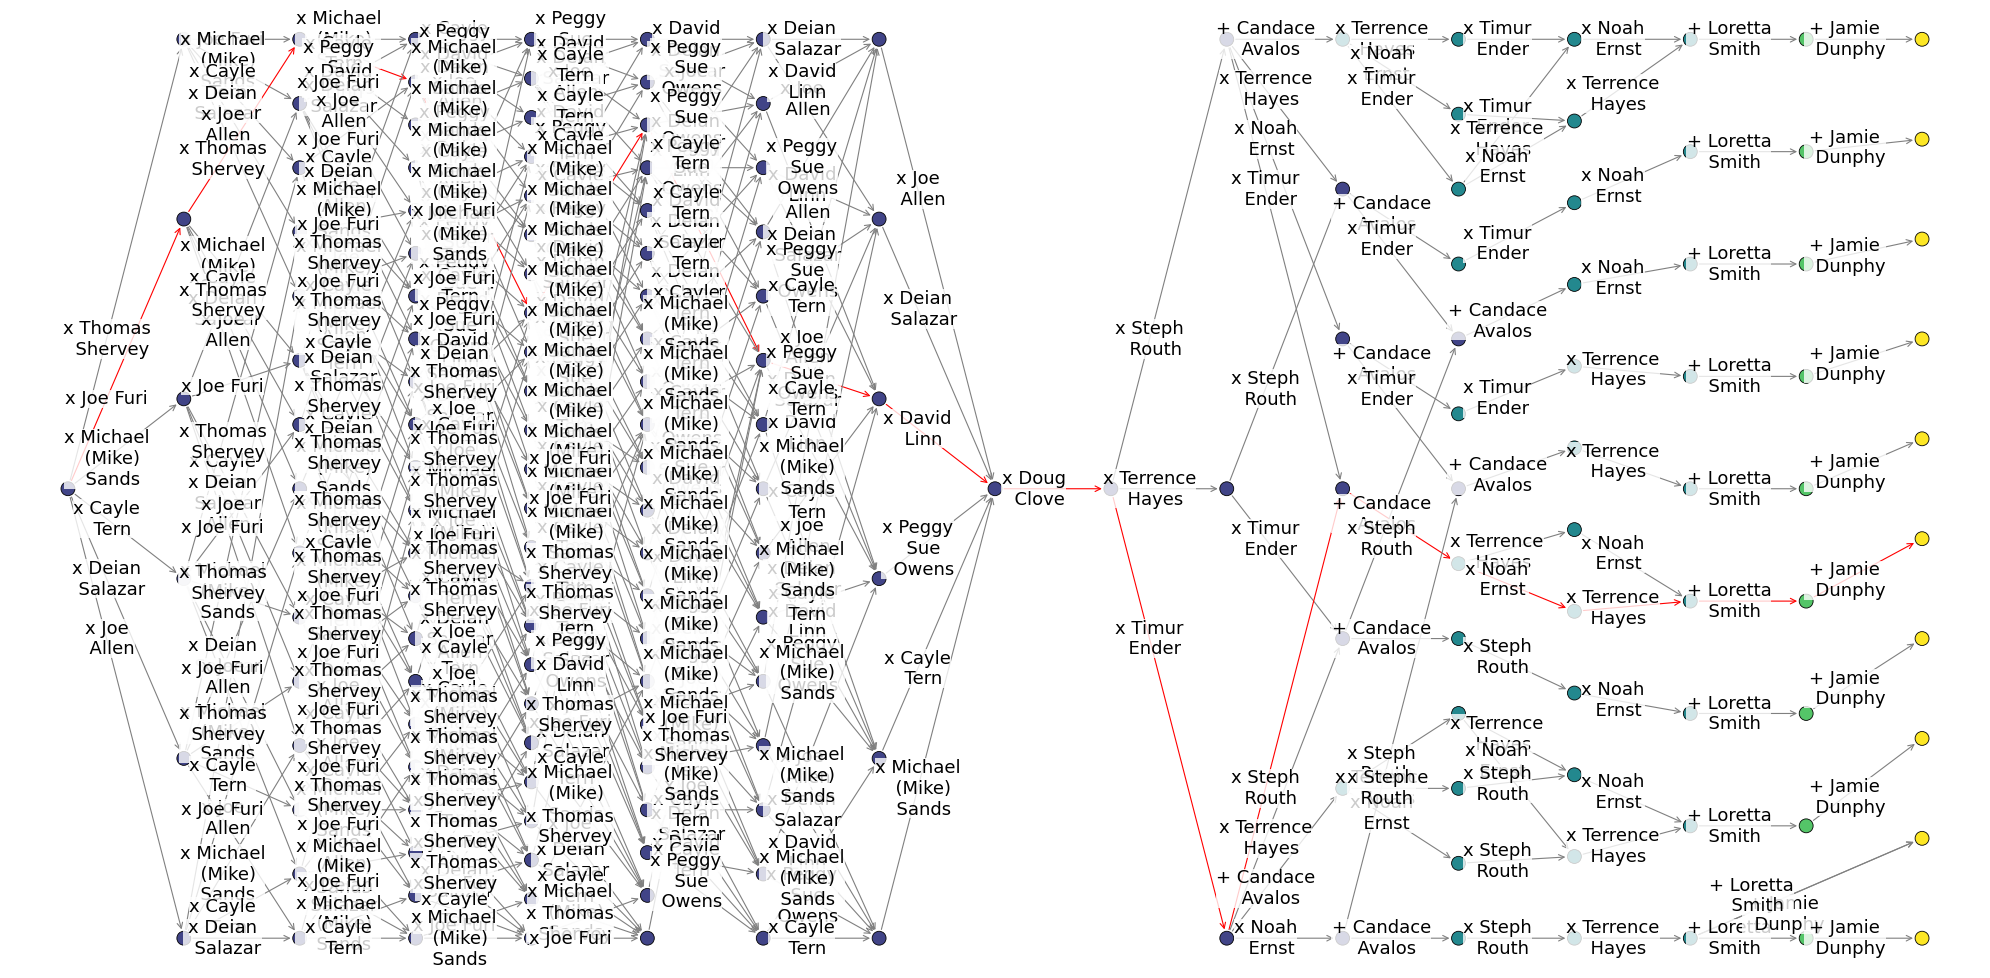
\includegraphics[width=\textwidth]{graphics/portland_d1.png}
    \caption{A coherent and plausible graph for a 2024 3-seat STV election in Portland, OR. This election had $C=16$ candidates, $m=3$ seats, $N=42,678$ ballots, and the graph was constructed with a margin of $M=671$. The vertices are color-coded by degree, and the natural path is highlighted in red.}
    \label{fig:portland_d1}
\end{figure}

\subsection{Shortcuts for Larger Elections.}\label{sec:shortcut}

With larger candidate counts, the computation of a full plausible graph becomes computationally intractable.
The early layers of the audit graphs are especially prone to combinatorial explosion, as there tends to be a large set of ``weak candidates'' whose elimination is plausible at any stage of the election. 

This pattern already emerges in Figure \ref{fig:portland_d1}, where layers 0 through 7 of the graph contain $111/175$ of the vertices of the graph, and it is further accentuated for larger elections, where the first half of the graph's layers routinely contain more than $90\%$ of the vertices.

We can leverage some systematic patterns from real world data to mitigate this combinatorial explosion.
For example, strong candidates tend to start strong and remain so throughout in real world elections, unlike the pathological examples which imagine ``dark horse'' winners always on the brink of elimination.
In this setting, it is possible to abridge the early layers of a plausible graph by using a ``batch elimination'' which rigorously justifies the simultaneous elimination of all candidates in a designated weak set. 

To justify a batch elimination, we fix a Margin of Insecurity $M$, and we distinguish two disjoint subsets $\VS, \SSS\subset \CCC$ of \emph{Very Strong} and \emph{Strong} candidates.

The (possibly empty) set $\VS$ consists of those candidates who make quota by more than a $M$ votes on initial preferences, or upon receiving transfers from other very strong candidates. 
In other words, these are the candidates who will be seated before anything else happens in the plausible graph: any path from the root to a leaf of the plausible graph must initially follow a sequence of seating edges corresponding to very strong candidates.
We call the possibly multiple vertices where all very strong candidates are seated and no other candidates were eliminated or seated the \emph{base vertices} of the batch eliminations.

The set $\SSS$ of strong candidates can be chosen arbitrarily, but it induces a \emph{Weak Set} $\LLL\subseteq \CCC$ on each base vertex, and in practice it will be desirable to pick $\SSS$ so as to make $\LLL$ as large as possible.
We say a candidate $l\in \CCC$ is \emph{weak} with respect to $\SSS$ in the base vertex $\ov$ if her \emph{Maximum Possible Tally} ($\MPT$) is lower than the smallest tally of a strong candidate according to $\ov$.
Informally, we count any ranking which mentions $l$ before any strong candidate in $\SSS$ as giving its full weight in $\ov$ to $\MPT(l)$.

After computing the weak set $\LLL$, we are left with a set $\OOO = \CCC - (\VS\cup\SSS\cup\LLL)$ of \emph{Other} candidates which fell into none of the previous categories.

If we verify that none of the strong candidates can possibly make quota before all of the weak candidates are eliminated, the above definitions guarantee that any plausible path must at some point visit a vertex descended from a base vertex whose hopeful set contains all of $\SSS$ and some subset $\OOO'\subseteq \OOO$.
So we may abridge the process of plausible graph construction by seeding it with the set of all such vertices, rather than the root vertex.

\begin{figure}
    \centering
    
\includegraphics[width=\textwidth]{"graphics/vic_2025.png"}
\caption{Plausible and coherent graph for a 6-seat STV election for Federal Senate in Victoria, Australia. For this graph, $N=4,101,762$, $M=23,000$, $C = 65$, $|\VS|=4$, $|\SSS|=9$, $|\LLL|=42$, and $|\OOO|=10$, meaning there were $2^{10}=1024$ seeded vertices after the batch elimination, which is indicated in the graph by a vertical black bar.}
    \label{fig:vic}
\end{figure}

To encode the requirement that no strong candidate makes quota until all weak candidates are eliminated at the stage of graph construction, it is sufficient to verify that the tallies of all strong candidates are at least $M$ below quota in the vertex $\ou$ descended from the base vertex $\ov$ with $\HHH(\ou) = \SSS$ and $\lambda_{\ou} = \lambda_{\ov}$.
This requirement, like the weakness of all $l\in\LLL$, is contigent on a critical margin which is purely vertex-local to either $\ov$ or $\ou$, meaning they can be formulated into assertions that are auditable by the methods in \S\ref{sec:mismatch} or \S\ref{sec:delta}.
